\documentclass[conference]{IEEEtran}
\IEEEoverridecommandlockouts
% The preceding line is only needed to identify funding in the first footnote. If that is unneeded, please comment it out.
\usepackage{cite}
\usepackage{amsmath,amssymb,amsfonts}
\usepackage{algorithmic}
\usepackage{graphicx}
\usepackage{textcomp}
\usepackage{xcolor}
\def\BibTeX{{\rm B\kern-.05em{\sc i\kern-.025em b}\kern-.08em
    T\kern-.1667em\lower.7ex\hbox{E}\kern-.125emX}}
\begin{document}

\title{Auto Encoders and Gray level co-occurrence matrix for obstacle detection on railway tracks}

\author{\IEEEauthorblockN{Jeethesh Pai Umesh}
\IEEEauthorblockA{\textit{Technical University of Braunschweig} \\
Braunschweig, Germany \\
j.umesh@tu-braunschweig.de}
\and
\IEEEauthorblockN{Kanwal Jahan}
\IEEEauthorblockA{\textit{Institute for Transportation Systems} \\
\textit{German Aerospace Centre}\\
Braunschweig, Germany \\
jahan.kanwal@dlr.de}
\and
\IEEEauthorblockN{Michael Roth}
\IEEEauthorblockA{\textit{Institute for Transportation Systems} \\
\textit{German Aerospace Centre}\\
Braunschweig, Germany \\
michael.roth@dlr.de}
}

\maketitle

\begin{abstract}
This paper describes a way to identify obstacles on the railway tracks with the help of computer vision procedures. Auto encoder and gray level co-occurrence matrix is used to extract feature out of the image and classify it as outlier if it really is.
\end{abstract}

\begin{IEEEkeywords}
Semantic segmentation, auto encoders, gray level co-occurrence matrix, deep learning
\end{IEEEkeywords}

\section{Introduction}
Railway safety and accident prevention has been one of the primary task to ensure minimal loss and uninterrupted operations especially with high speed trains. We plan to detect obstacles which can/pose a threat to the safe functioning of the railways ahead of the accident. This technology when integrated with the warning system can help alleviate possible accidents.

\section{RELATED WORKS}

\subsection{Maintaining the Integrity of the Specifications}

The IEEEtran class file is used to format your paper and style the text. All margins, 
column widths, line spaces, and text fonts are prescribed; please do not 
alter them. You may note peculiarities. For example, the head margin
measures proportionately more than is customary. This measurement 
and others are deliberate, using specifications that anticipate your paper 
as one part of the entire proceedings, and not as an independent document. 
Please do not revise any of the current designations.

\section{PROPOSED METHOD}
Our method detects the obstacles or anomalies along the track with the help of deep learning methods. First, we try to sketch out rails from the given image which will be inspected later on for anomaly presence. We perform a semantic segmentation here with rail track as class labelled 1 and non-rail classes labelled 0. We use the model U-Net \cite{ronneberger2015unet} for semantic segmentation task. This model has skip connections (copy and crop) throughout its stream so as to prevent lossy compression by the pooling layer. During each pooling, a copy of feature map is stored for later concatenation that can help avoid better edge approximations. The concatenation of old feature maps preserves spatial feature when compared to pooled layers and pooled layers extracts features which are essential for semantic segmentation task. The ``Fig.~\ref{U-Net}'' shows the architecture of our semantic segmentation model.
\begin{figure}[htbp]
\centerline{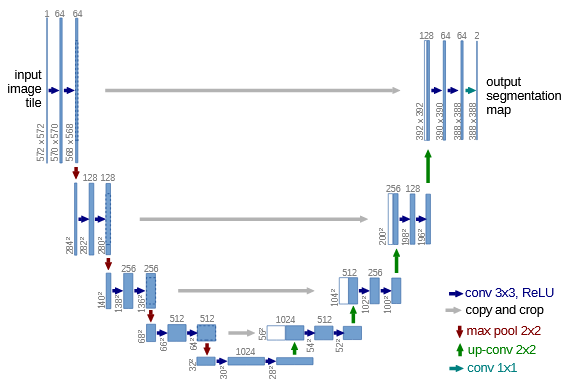
\includegraphics[height=6.5cm]{U-Net_model.png}}
\caption{U-Net architecture Overview}
\label{U-Net}
\end{figure} 


The U-Net network is used to semantically segments the rail lines from the given railway image. Once the rail coordinates from the image data is known, next step is to extract the features along the above-mentioned rail coordinates. To extract feature, as a first step we group out the pixel coordinates which belong to left rail, right rail separately. If there are more rails in an image, then care is taken so that rail pixel coordinates are not mismatched. Then one of the rail lines is selected and a rectangular patch of variable breadth is used to extract feature on that particular part of rail. See ´´Fig.~\ref{Rail_line} for more details. 
\begin{figure}[htbp]
\centerline{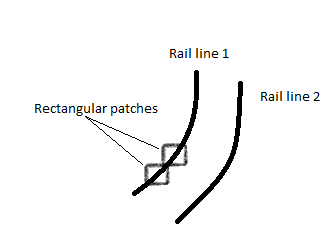
\includegraphics[height=4cm]{Rail_line_illustration.png}}
\caption{Extracting features along the rail line}
\label{Rail_line}
\end{figure} 
We extract features of each rectangular patch along the same rail line and check if there are anomalies along the same rail. The idea is, whenever some obstacle or non-rail objects come along the rail line, it will block some part of the rail line which will trigger a different feature for that part of rail. For feature extraction, we use Auto-encoders and Gray level co-occurrence matrix. The auto-encoders are neural networks which helps to extract hidden information from a given image unlike hand crafted features. The Auto-encoder has an encoder-decoder structure. The encoder structure ensures that the image fed in is converted into compressed form. Even though, the latent space dimension, which is generated at the end of encoder part of the model, is high, when compared to input image dimension. This quantity is significantly lower and can represent the given input image in a lower dimension effectively. From here the decoder tries to reconstruct the input image given the latent space. This reconstruction error is back-propagated to train the weights. The loss function used here is mean squared error (MSE). We train with the patches of rail generated from RO-DLR dataset [RO DLR Dataset YouTube video reference]. we use the best weight to calculate the reconstruction error of each patch for prediction of anomalies. If the reconstruction error is smaller, then the observed rectangular patch is similar to the one which auto encoder was trained on and hence there is no anomaly. When the reconstruction error is large, it means there is a presence of obstacle in the observed rectangular patch and hence is classified as anomaly. In order to classify the array of reconstruction error values, obtained by dividing the rail into multiple patches we use thresholding. We first do a K means clustering of 2 on the array and check whether the difference in cluster center values is greater than threshold or not. After trial and error, the threshold value was found to be 0.40. If the difference in cluster value is found to be greater than threshold, then the cluster center with larger reconstruction error is considered as anomaly and furthermore its locations are also marked showing as anomaly.


\section{Experiments}
\begin{itemize}
\item We start the training with semantic segmentation of rail lines from the background. U-Net is chosen as per \cite{ronneberger2015unet} description. The data used here is Railsem-19 \cite{9025646}  which is publicly available. Railsem-19 data contains total of 8500 images with semantic labels mapped on to json files. We split the data into 8390 training images, 60 validation images and 50 test images. We use Tensorflow \cite{tensorflow2015-whitepaper} backend throughout the pipeline. Training was done with 2 NVIDIA GeForce GTX 1080 Ti GPU's with a batch size of 2 and image size of 512 x 512 x 3 (RGB image) as input. We use focal loss \cite{lin2018focal} to train our network since there is a large imbalance of foreground and background pixels in the data set. Focal loss penalizes more for errors on foreground pixels. As per the focal loss \ref{focalloss} equation the loss
\begin{equation} 
    FL(p_{t})=-\alpha( 1 - p_{t})^{\gamma}log(p_{t})
\end{equation}\label{focalloss}
 where,
 
 p\textsubscript{t} = model's estimated probability for the foreground class
 
 
 $\alpha$ = penalty for foreground error (treats imbalance of foreground and background)
 
 
 $\gamma$ = modulation factor for easy and hard classifications
 
 
\item Auto encoder training was done for 50 epochs with a learning rate of 0.0001. After training we choose the best weight of Auto encoder to reconstruct the rail patch of the test image.
\item Do not mix complete spellings and abbreviations of units: ``Wb/m\textsuperscript{2}'' or ``webers per square meter'', not ``webers/m\textsuperscript{2}''. Spell out units when they appear in text: ``. . . a few henries'', not ``. . . a few H''.
\item Use a zero before decimal points: ``0.25'', not ``.25''. Use ``cm\textsuperscript{3}'', not ``cc''.)
\end{itemize}

\subsection{Equations}
Number equations consecutively. To make your 
equations more compact, you may use the solidus (~/~), the exp function, or 
appropriate exponents. Italicize Roman symbols for quantities and variables, 
but not Greek symbols. Use a long dash rather than a hyphen for a minus 
sign. Punctuate equations with commas or periods when they are part of a 
sentence, as in:
\begin{equation}
a+b=\gamma\label{eq}
\end{equation}

Be sure that the 
symbols in your equation have been defined before or immediately following 
the equation. Use ``\eqref{eq}'', not ``Eq.~\eqref{eq}'' or ``equation \eqref{eq}'', except at 
the beginning of a sentence: ``Equation \eqref{eq} is . . .''

\subsection{\LaTeX-Specific Advice}

Please use ``soft'' (e.g., \verb|\eqref{Eq}|) cross references instead
of ``hard'' references (e.g., \verb|(1)|). That will make it possible
to combine sections, add equations, or change the order of figures or
citations without having to go through the file line by line.

Please don't use the \verb|{eqnarray}| equation environment. Use
\verb|{align}| or \verb|{IEEEeqnarray}| instead. The \verb|{eqnarray}|
environment leaves unsightly spaces around relation symbols.

Please note that the \verb|{subequations}| environment in {\LaTeX}
will increment the main equation counter even when there are no
equation numbers displayed. If you forget that, you might write an
article in which the equation numbers skip from (17) to (20), causing
the copy editors to wonder if you've discovered a new method of
counting.

{\BibTeX} does not work by magic. It doesn't get the bibliographic
data from thin air but from .bib files. If you use {\BibTeX} to produce a
bibliography you must send the .bib files. 

{\LaTeX} can't read your mind. If you assign the same label to a
subsubsection and a table, you might find that Table I has been cross
referenced as Table IV-B3. 

{\LaTeX} does not have precognitive abilities. If you put a
\verb|\label| command before the command that updates the counter it's
supposed to be using, the label will pick up the last counter to be
cross referenced instead. In particular, a \verb|\label| command
should not go before the caption of a figure or a table.

Do not use \verb|\nonumber| inside the \verb|{array}| environment. It
will not stop equation numbers inside \verb|{array}| (there won't be
any anyway) and it might stop a wanted equation number in the
surrounding equation.

\subsection{Some Common Mistakes}\label{SCM}
\begin{itemize}
\item The word ``data'' is plural, not singular.
\item The subscript for the permeability of vacuum $\mu_{0}$, and other common scientific constants, is zero with subscript formatting, not a lowercase letter ``o''.
\item In American English, commas, semicolons, periods, question and exclamation marks are located within quotation marks only when a complete thought or name is cited, such as a title or full quotation. When quotation marks are used, instead of a bold or italic typeface, to highlight a word or phrase, punctuation should appear outside of the quotation marks. A parenthetical phrase or statement at the end of a sentence is punctuated outside of the closing parenthesis (like this). (A parenthetical sentence is punctuated within the parentheses.)
\item A graph within a graph is an ``inset'', not an ``insert''. The word alternatively is preferred to the word ``alternately'' (unless you really mean something that alternates).
\item Do not use the word ``essentially'' to mean ``approximately'' or ``effectively''.
\item In your paper title, if the words ``that uses'' can accurately replace the word ``using'', capitalize the ``u''; if not, keep using lower-cased.
\item Be aware of the different meanings of the homophones ``affect'' and ``effect'', ``complement'' and ``compliment'', ``discreet'' and ``discrete'', ``principal'' and ``principle''.
\item Do not confuse ``imply'' and ``infer''.
\item The prefix ``non'' is not a word; it should be joined to the word it modifies, usually without a hyphen.
\item There is no period after the ``et'' in the Latin abbreviation ``et al.''.
\item The abbreviation ``i.e.'' means ``that is'', and the abbreviation ``e.g.'' means ``for example''.
\end{itemize}
An excellent style manual for science writers is.

\subsection{Authors and Affiliations}
\textbf{The class file is designed for, but not limited to, six authors.} A 
minimum of one author is required for all conference articles. Author names 
should be listed starting from left to right and then moving down to the 
next line. This is the author sequence that will be used in future citations 
and by indexing services. Names should not be listed in columns nor group by 
affiliation. Please keep your affiliations as succinct as possible (for 
example, do not differentiate among departments of the same organization).

\subsection{Identify the Headings}
Headings, or heads, are organizational devices that guide the reader through 
your paper. There are two types: component heads and text heads.

Component heads identify the different components of your paper and are not 
topically subordinate to each other. Examples include Acknowledgments and 
References and, for these, the correct style to use is ``Heading 5''. Use 
``figure caption'' for your Figure captions, and ``table head'' for your 
table title. Run-in heads, such as ``Abstract'', will require you to apply a 
style (in this case, italic) in addition to the style provided by the drop 
down menu to differentiate the head from the text.

Text heads organize the topics on a relational, hierarchical basis. For 
example, the paper title is the primary text head because all subsequent 
material relates and elaborates on this one topic. If there are two or more 
sub-topics, the next level head (uppercase Roman numerals) should be used 
and, conversely, if there are not at least two sub-topics, then no subheads 
should be introduced.

\subsection{Figures and Tables}
\paragraph{Positioning Figures and Tables} Place figures and tables at the top and 
bottom of columns. Avoid placing them in the middle of columns. Large 
figures and tables may span across both columns. Figure captions should be 
below the figures; table heads should appear above the tables. Insert 
figures and tables after they are cited in the text. Use the abbreviation 
``Fig.~\ref{fig}'', even at the beginning of a sentence.

\begin{table}[htbp]
\caption{Table Type Styles}
\begin{center}
\begin{tabular}{|c|c|c|c|}
\hline
\textbf{Table}&\multicolumn{3}{|c|}{\textbf{Table Column Head}} \\
\cline{2-4} 
\textbf{Head} & \textbf{\textit{Table column subhead}}& \textbf{\textit{Subhead}}& \textbf{\textit{Subhead}} \\
\hline
copy& More table copy$^{\mathrm{a}}$& &  \\
\hline
\multicolumn{4}{l}{$^{\mathrm{a}}$Sample of a Table footnote.}
\end{tabular}
\label{tab1}
\end{center}
\end{table}

\begin{figure}[htbp]
\centerline{
\includegraphics{fig1.png}}
\caption{Example of a figure caption.}
\label{fig}
\end{figure}

Figure Labels: Use 8 point Times New Roman for Figure labels. Use words 
rather than symbols or abbreviations when writing Figure axis labels to 
avoid confusing the reader. As an example, write the quantity 
``Magnetization'', or ``Magnetization, M'', not just ``M''. If including 
units in the label, present them within parentheses. Do not label axes only 
with units. In the example, write ``Magnetization (A/m)'' or ``Magnetization 
\{A[m(1)]\}'', not just ``A/m''. Do not label axes with a ratio of 
quantities and units. For example, write ``Temperature (K)'', not 
``Temperature/K''.

\section*{Acknowledgment}

The preferred spelling of the word ``acknowledgment'' in America is without 
an ``e'' after the ``g''. Avoid the stilted expression ``one of us (R. B. 
G.) thanks $\ldots$''. Instead, try ``R. B. G. thanks$\ldots$''. Put sponsor 
acknowledgments in the unnumbered footnote on the first page.

\section{References}

Please number citations consecutively within brackets. The 
sentence punctuation follows the bracket . Refer simply to the reference 
number, as in  '---do not use ``Ref.  ''' or ``reference  ''' except at 
the beginning of a sentence: ``Reference  ' was the first $\ldots$''

Number footnotes separately in superscripts. Place the actual footnote at 
the bottom of the column in which it was cited. Do not put footnotes in the 
abstract or reference list. Use letters for table footnotes.

Unless there are six authors or more give all authors' names; do not use 
``et al.''. Papers that have not been published, even if they have been 
submitted for publication, should be cited as ``unpublished''   . Papers 
that have been accepted for publication should be cited as ``in press''  . 
Capitalize only the first word in a paper title, except for proper nouns and 
element symbols.

For papers published in translation journals, please give the English 
citation first, followed by the original foreign-language citation

\bibliographystyle{IEEEtran}
\addcontentsline{toc}{section}{References}
\bibliography{main}

\vspace{12pt}
\color{red}
IEEE conference templates contain guidance text for composing and formatting conference papers. Please ensure that all template text is removed from your conference paper prior to submission to the conference. Failure to remove the template text from your paper may result in your paper not being published.

\end{document}
